\documentclass[conference]{IEEEtran}
\IEEEoverridecommandlockouts
% The preceding line is only needed to identify funding in the first footnote. If that is unneeded, please comment it out.
\usepackage{cite}
\usepackage{float}
\usepackage{amsmath,amssymb,amsfonts}
\usepackage{graphicx}
\usepackage{textcomp}
\usepackage{xcolor}
\def\BibTeX{{\rm B\kern-.05em{\sc i\kern-.025em b}\kern-.08em
    T\kern-.1667em\lower.7ex\hbox{E}\kern-.125emX}}
\begin{document}

\title{CENG435-DATA COMMUNICATIONS AND NETWORKING \\ TERM PROJECT PHASE-2 REPORT
{\footnotesize}
\thanks{}
}

\author{\IEEEauthorblockN{ Ahmet Dara VEFA}
\IEEEauthorblockA{\textit{2237899} \\
\textit{Group-68}
}
\and
\IEEEauthorblockN{ Alper KOCAMAN}
\IEEEauthorblockA{\textit{2169589} \\
\textit{Group-68}
}
}

\maketitle

\section{Design and Implementation Part}
\subsection{Project Overview}
The purpose of this project is creating a reliable data transfer protocol(which is based on UDP) that also uses multi-homing and pipelining. \\
Multi-homing is the transfer of data from multiple channels/links and pipelining is receiving data while sending the previously received data. \\
There is a source node that has the file we need to transfer(input.txt) which is connected to 3 routers(r1,r2,r3) and the routers are also connected to destination node. We need to transfer input.txt from source to destination with our own RDT protocol. You can find more information about our RDT protocol in the design approach section. \\
We are required to run 2 experiments. In the first one we will send the file along the shortest path which is Source-R3-Destination. In the second experiment we will send the file along the remaining routers which is Source-R1\&R2-Destination. During experiment 2 one of the links between source and r1 or r2 may be down so we should be able to handle down links. \\
While designing our protocol we ran into some ideological problems like using go-back-N or selective repeat methods and talked about it before designing, you can find more details about this in the design approach and implementation approach sections.
%%%%% NOTE:  we can talk about experiments delay etc. in here or something

\subsection{Design Approach}
We needed to transfer a file of 5 MBytes from source to destination. Since max packet size is 1500bytes(including 20 bytes for header) we needed to divide the file into smaller packets. \\
We chose packet size to be maximum 900 bytes(including headers) since around 800-900 bytes is the most reliable for UDP. \\
Since UDP is not reliable we needed to ensure our packets reached the destination. In case of a packet loss or md5 failure we needed a mechanism for re-sending the packets. \\
We first thought about implementing a torrent like structure where the destination would request the packets it needed from the routers and the routers would request the required packets from the source node. However later on we decided go-back-N would be easier to implement since it is a set in stone method that does not require us to re-invent the wheel. \\
%%%%% NOTE: hangi nodelarda hangi arrayler vs var niye var diye yazılabilir
The sent packets contain the packet's index, md5 checksum and data. We need to send the index since UDP does not guarantee that the packets will arrive in order and since we are using multi-homing we must know which packet belongs to where. We need to send md5 checksum along with the data itself since UDP does not guarantee that the data will arrive correctly.\\
We also have a timeout mechanism in the source node to ensure that lost packets are not causing the other nodes to wait for eternity in the event of a packet loss.\\
We first send the packet to a router then to a destination, after this we send the ACK messages back to router then to source. This is done because if we sent ACK to source when a router successfully acquired a packet source node would mark that packet as successfully sent to destination; therefore, in the event of a down link between router and destination, our source would not know about this and those packets that were sent to the node with broken link to destination would be stuck at router. \\
Replies contain ACK/NACK message and index of packet. We use the index to mark the packet as acquired by destination or to re-send the packet(along with rest of the window since we are using go-back-N) \\
\\
The general structure of the network is like this: Source reads the input.txt file, divides it into smaller packets, sends the first N(window size) packets to a router(also sends the last N packets to another router if applicable). Whenever a router receives the a packet it has not received(and when the other router receives the last packet if there are 2 routers), they save that packet to their respective array, which is used for sending the data to destination. When sender thread takes control it sends the packets that are not yet sent or has been timed out to destination. When destination receives the packet at the start of the window it will send ACK's for each of the consecutive received packets. \\ 
When a router receives an ACK for the next awaited packet it sends it back to source node along with the next packets that the node received ACK for. Then at source node if the next awaited ACK is received the window moves to the next node and on the bool array(at the ACK packet's index value) that index is marked as true. \\
Since there can be 2 active windows when a window moves to the next node it checks whether or not the packet at the new index is received by destination(from the bool array), if it is received by the destination the window will shrink, the source wont re-send that packet. \\
When the destination receives the last needed packet it closes its sockets. \\
When the source receives the last needed ACK packet it closes its sockets. \\
Routers don't close their sockets. \\

\subsection{Implementation Approach}
We decided to implement our design on python language since we already used python in part1 we felt more confident with python. \\ 
We read the input and divided it into chunks that could fit our target packet size(max 900 bytes). \\
We created a slice with instaGENI using the given topology xml and used the link information(ipv4 addresses) on that slice for creating sockets. \\
We knew that the functions would be really similar, so we started implementing the source node. Source node has a sender which sends the data and a listener for listening to ACK's coming from routers. Since source node has the input.txt file source node also has a function for reading the input and dividing it into smaller packets which contain the index of that packet, md5 checksum value of that data and finally the data itself. \\
We then implemented router nodes. Router node listens source node for data, listens to destination node for ACK messages, sends packets to destination and sends ACK messages to source. When new data comes router node checks its validity via recalculating md5 checksum. If validity is OK the packet gets sent to destination node. Destination node rechecks the validity of the packet via recalculating md5 checksum. If validity is OK at destination node, destination node sends an ACK message with the index of the packet to router(destination does this for all consecutive packets it received correctly). When router receives the ACK message it re-sends the message to source node. In source node that part of all the packets is marked as "received by destination", so it is not needed to resend that packet. \\
Lastly we implemented destination node. Destination node listens router(s) for packets and sends ACK messages to those routers. \\
When source node starts sending the packets of that window it starts a timer(0.5 seconds) for the first packet of that window. If the ACK message for the first packet does not come in a given time, source node re-sends the whole window again. \\
When destination node receives the last valid packet of the file, it creates the file from the saved data.\\


\section{Methodology and Motivation}
\subsection{Methodology}
Python hashlib library is used for generating md5 Checksums. \\
Python socket library is used for python socket API. \\
Python struct library is used for encoding messages. \\
Python time library is used for generating timestamps. \\
Python threading library is used for multithreading.


\subsection{Motivation}
In this project we learned how to make UDP reliable. We also learned how multi-homing and pipelining is implemented in networking. \\

\section{Experimental Results}
\subsection{Used Protocols and Tools For Experiment}
\textbf{Network Time Protocol}:
The first protocol that we have used in order to carry out experiment is NTP(Network Time Protocol).
Since the computer's internal times may be different from other computers in the same network, the internal time of each computer in the network should be made the same explicitly. NTP is used for this purpose. This protocol is intended to synchronize the computer clocks in a variable-latency, over packet-switched data networks. 

\textbf{Network Emulator}:
NetEm is an abbreviation of NEtwork EMulator. This emulator is employed in order to increase the Linux traffic control facilities. With the aid of NetEm, a selected network interface can be calibrated such that delay, packet loss, duplication and more other characteristics can be added to this interface's packets.\\
In the experiment part, this tool is used to emulating the delay on selected interfaces. These selected interfaces are: 
source to router1, router2 and router3 interfaces,\\
destination to router1, router2 and router3 interfaces,\\
router1 to source and destination interfaces,\\
router2 to source and destination interfaces,\\
router3 to source and destination interfaces.\\
The given delay for above mentioned interfaces are 3 milliseconds.\\
In this experiments, we applied not only delay to interfaces but also a packet loss percentages were applied to selected interfaces. These selected interfaces are above mentioned interfaces.\\
The applied packet loss percentages are $5$, $15$ and $38$.\\

\subsection{Experimental Part}

In the experiment part, mainly we have carried out 2 different experiments. Main task in these experiments were measuring end to end file transfer time between source node and destination node. Between these nodes for experiment 1, router 3 was used which had been found the shortest link between them in the first phase of the term project. This file transfer time (between source node and destination node) finding task should be done for 3 different packet loss percentages with 3ms network emulation delays. Thus, we have executed our script for firstly $5\%$ packet loss with 3ms network emulation delay , afterwards $15\%$ packet loss with 3ms network emulation delay and finally $38\%$ packet loss with 3ms network emulation delay.\\
In order to emulate special delays between the nodes, scripts that have NetEm commands are used. We'll explain these commands briefly in below.\\
For source node, firstly we need to find the interface name which links the source and router3. When we typed the "ifconfig" command in the terminal of source, all interfaces and their names were shown as well as their IP addresses. We found out that the interface whose IP address is "10.10.3.1" links the source with router3. The name of this interface was "eth3". Then we executed the below script for both applying packet loss percentages and network emulation delay\\
"tc qdisc add dev eth3 root netem loss $5\%$ delay 3ms "\\
We couldn't use the given:\\
tc qdisc change dev [INTERFACE] root netem loss $5\%$ delay 3ms\\ command since it is need sudo permissions. When we tried to do with sudo  mode, it gave the file not exist error.\\
Like applied command to source-router3 link, we applied the needed commands for other interfaces. Interface needed to be applied NetEm commands are:\\
source-router3,\\
router3 - source,\\
destination-router3,\\
router3-destination\\
for the first experiment.\\
After these commands are applied to above mentioned interfaces, we put all the implemented scripts. We put these scripts in a seperated directory whose name is "source-r3-dest scripts". We put these scripts in the relevant nodes in our topology. Their names are source.py, router3.py and destination.py in the remotes.\\
Then we executed all the scripts in their terminals. However, since the scripts should be executed for a considerable amount in order to get meaningful results, we executed all the scripts for 10 times. \\
One of the results are shown below,

\begin{figure}[H]
    \centering
    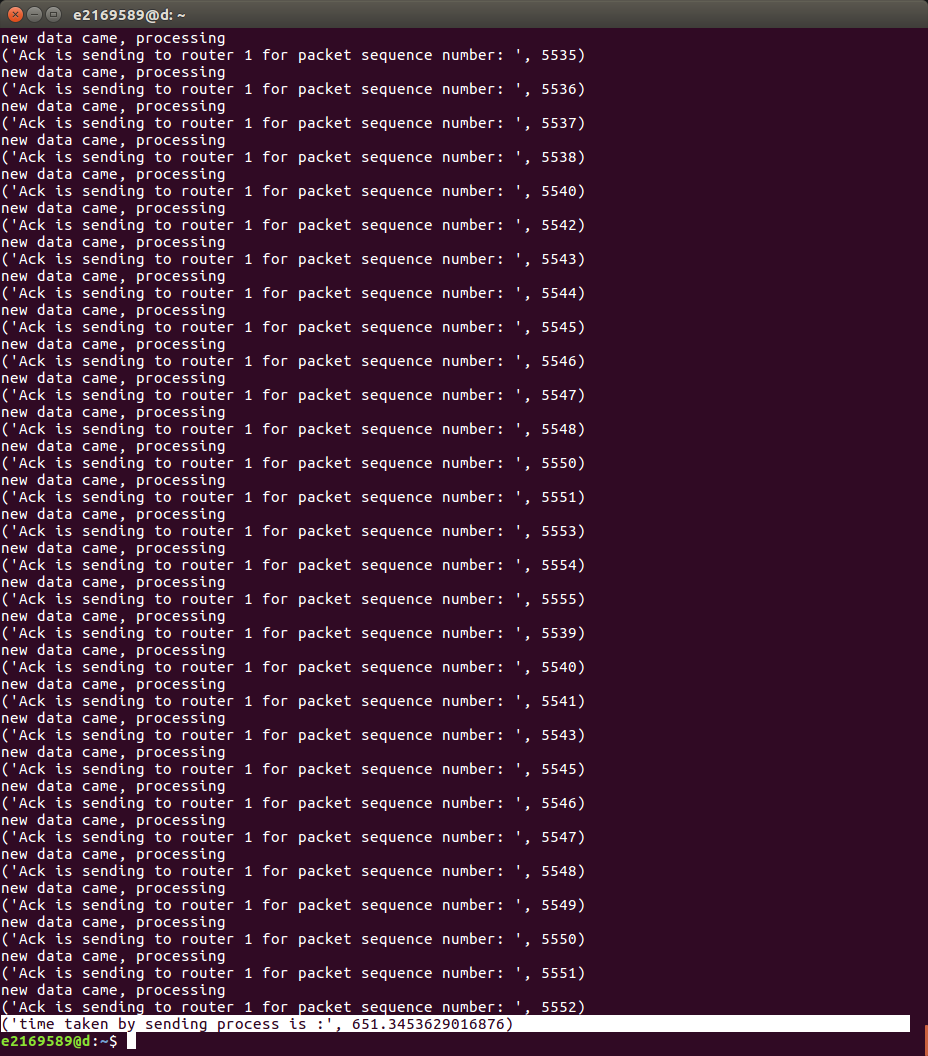
\includegraphics[scale=0.13]{5loss.png}
    \caption{Example from one of the executions for $5\%$ loss}
\end{figure}

We put here other results as well for experiment1 with $5\%$ loss:

\begin{table}[H]
\begin{tabular}{|l|l|}
\hline
Trial Number & Total Time \\ \hline
1            & 654.207    \\ \hline
2            & 648.387    \\ \hline
3            & 651.908    \\ \hline
4            & 646.200    \\ \hline
5            & 649.561    \\ \hline
6            & 653.325    \\ \hline
7            & 650.869    \\ \hline
8            & 646.453    \\ \hline
9            & 648.537    \\ \hline
10           & 653.841    \\ \hline
\end{tabular}
\end{table}

After doing first part of the first experiment, we continued with second part which is same delay on the same nodes but with $15\%$ loss. Like explained in the above, we needed to find the related interfaces and their names. We applied \\
"tc qdisc add dev [Interface] root netem loss $15\%$ delay 3ms "\\ command for below interfaces:\\
source-router3,\\
router3 - source,\\
destination-router3,\\
router3-destination.\\
But before applying this command to change the packet loss to 15, we needed another command because we get another error like this file already exist. Thus we needed to execute following command:\\
"tc qdisc del dev [Interface] root".\\
The interface variable was usually "eth3".\\
Then we executed all the scripts in their terminals. However, since the scripts should be executed for a considerable amount in order to get meaningful results, we executed all the scripts for 10 times. \\
One of the results are shown below,

\begin{figure}[H]
    \centering
    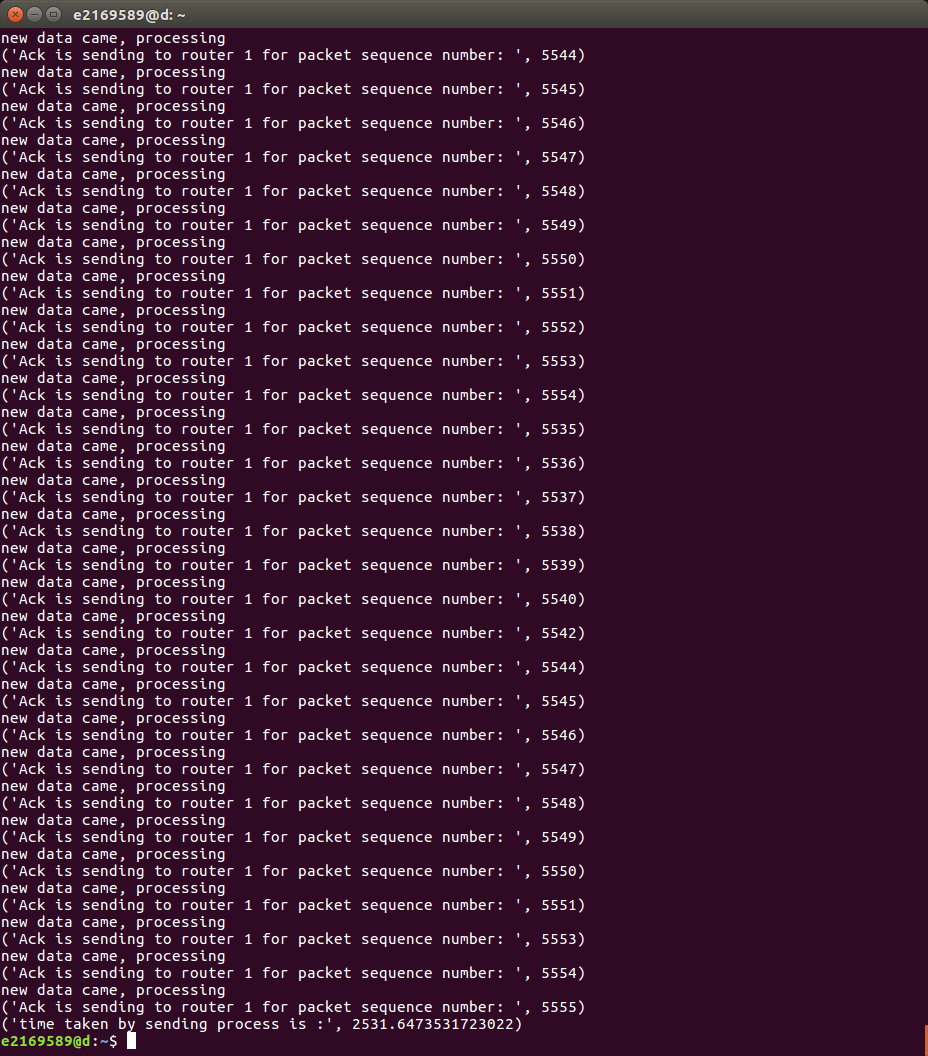
\includegraphics[scale=0.13]{15loss.png}
    \caption{Example from one of the executions for $15\%$ loss }
\end{figure}

We put here other results as well for experiment1 with $15\%$ loss:
\\
\begin{table}[H]
\begin{tabular}{|l|l|}
\hline
Trial Number & Total Time \\ \hline
1            & 2531.647   \\ \hline
2            & 2538.851   \\ \hline
3            & 2529.548   \\ \hline
4            & 2540.489   \\ \hline
5            & 2538.316   \\ \hline
6            & 2534.169   \\ \hline
7            & 2528.963   \\ \hline
8            & 2525.691   \\ \hline
9            & 2534.167   \\ \hline
10           & 2539.496   \\ \hline
\end{tabular}
\end{table}

Since our results are high and we didn't want to wait, we opened this scripts and the results were written to a file by scripts.\\\\
Lastly, we continued with the third part. This part was needed to apply $38\%$ packet loss with same emualtion delay, which is 3 milliseconds.\\
Like explained in the above 2 parts, we needed to find the related interfaces and their names. We applied \\
"tc qdisc add dev [Interface] root netem loss $38\%$ delay 3ms \\ command for related interfaces.\\
But before applying this command to change the packet loss to 38, we needed another command because we get another error like this file already exist. Thus we needed to execute following command:\\
"tc qdisc del dev [Interface] root".\\
The interface variable was usually "eth3".\\
Then we executed all the scripts in their terminals. However, since this time, it takes huge amount of time, we only run scripts with this configuration 1 times. The result was 8532.620. \\\\
Also, before starting, we did the experiment without appliying any delay and packet loss with NetEm. As it easily guessed, the fastest one is this. One of the results are like this,

\begin{figure}[H]
    \centering
    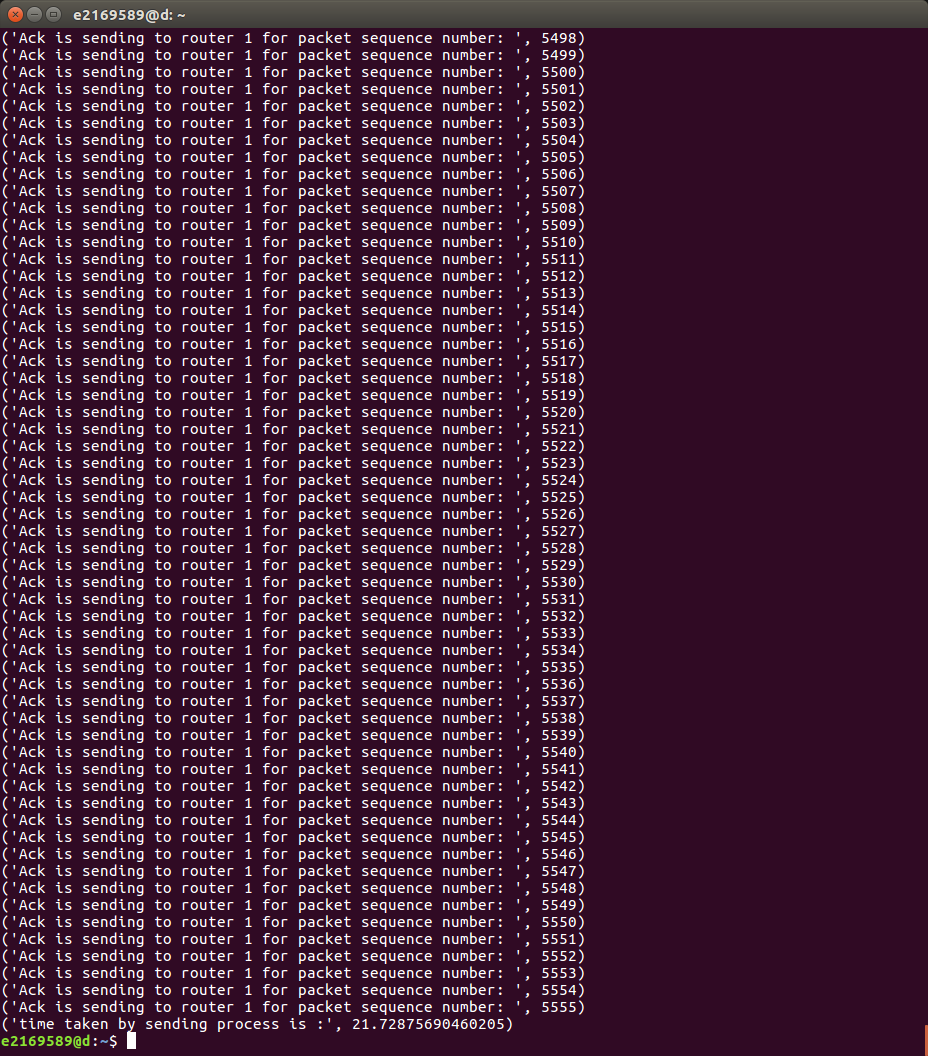
\includegraphics[scale=0.13]{0loss.png}
    \caption{Example from one of the executions for $0\%$ loss }
\end{figure}

At this point, we have finished the first experiment and ready to start other experiment. These are the average results for first experiment.\\

\begin{table}[H]
\begin{tabular}{|l|l|}
\hline
Loss(percentage) & Average Time To Finish(s) \\ \hline
0                & 21.728                    \\ \hline
5                & 651.345                   \\ \hline
15               & 2531.647                  \\ \hline
38               & 8532.620                  \\ \hline
\end{tabular}
\end{table}

In the second part of the experiment part, main task is the same with the first experiment. Main task in these experiments were measuring end to end file transfer time between source node and destination node. However in the second part of the experiment, between source node and destination node, router 1 and router 2  were used. These routers were configured in the first part of the term project. This file transfer time (between source node and destination node) finding task had been done for 1 packet loss percentage which is $5\%$. Also, there exists 3ms network emulation delay. Thus, we have executed our script for $5\%$ packet loss with 3ms network emulation delay.\\
In order to emulate special delays between the nodes, scripts that have NetEm commands were used. We'll explain these commands briefly in below.\\
For source node, firstly we need to find the interface name which links the source and both router 1 and router 2. When we typed the "ifconfig" command in the terminal of source, all interfaces and their names were shown as well as their IP addresses. We found out that the interface whose IP addresses are "10.10.1.1" and "10.10.2.2" link the source with routers. The name of this interfaces were "eth1" and "eth2". Then we executed the below script for both applying packet loss percentages and network emulation delay\\
"tc qdisc add dev eth3 root netem loss $5\%$ delay 3ms "\\
We applied this command to other necessary interfaces. Interfaces needed to be applied NetEm commands are:\\
source-router1,\\
source-router2,\\
router1 - source,\\
router2 - source,\\
destination-router1,\\
destination-router2,\\
router1-destination\\
router2-destination\\
for the second experiment.\\
After these commands are applied to above mentioned interfaces, we put all the implemented scripts. We put these scripts in a seperated directory whose name is "source-r1\&r2-dest scripts". Script names are source2.py, router1.py, router2.py and destination2.py in the remotes.(There are 2 scripts in the source and destination nodes)\\
Then we executed all the scripts in their terminals. However, since the scripts should be executed for a considerable amount in order to get meaningful results, we executed all the scripts for 10 times. \\
One of the results like this,

\begin{figure}[H]
    \centering
    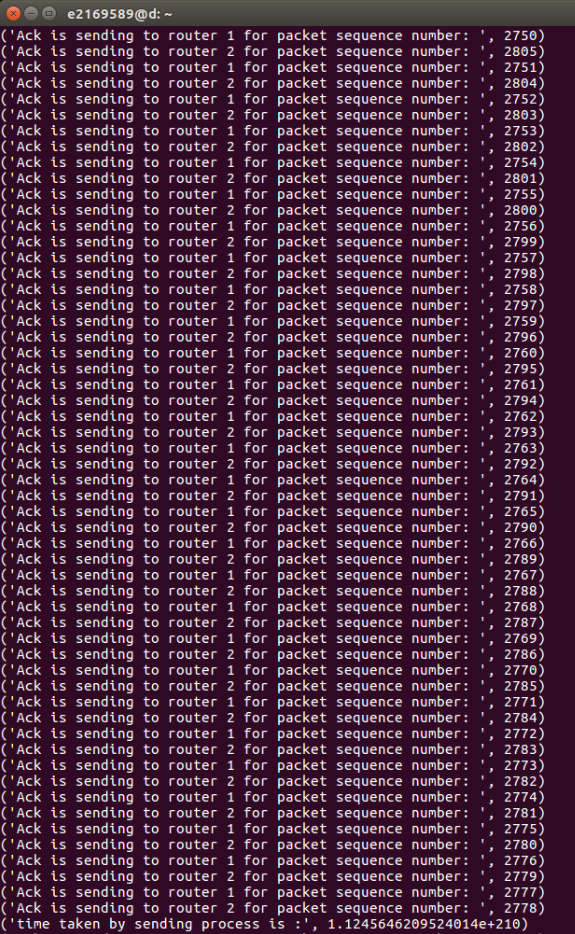
\includegraphics[scale=0.13]{exp2.png}
    \caption{Example from one of the executions for $5\%$ loss}
\end{figure}

All 10 results are shown in the below table,

\begin{table}[H]
\begin{tabular}{|l|l|}
\hline
Trial Number & Total Time \\ \hline
1            & 551.616    \\ \hline
2            & 554.961    \\ \hline
3            & 549.064    \\ \hline
4            & 547.319    \\ \hline
5            & 548.178    \\ \hline
6            & 551.456    \\ \hline
7            & 554.154    \\ \hline
8            & 552.105    \\ \hline
9            & 550.641    \\ \hline
10           & 553.310    \\ \hline
\end{tabular}
\end{table}

As can be seen in the screenshot, we sent packets according to their sequence number. If the sequence numbers of packets beginning from 0 to n, we sent these packet through router 1. If these packets sequence numbers are between n and 5555(last sequence number), we sent these packets through router 2. N is approximately midpoint of $[0,5555]$ interval.

As we mentioned previously, we sent a file from source to destination with size of 5 megabytes. In all cases, our destination script has achieved to open and write incoming packets into a file. When we checked the md5 checksum of the both files on the source and destination, they were same. Now we need to analyze results.  By looking these values, we collected the required information like standard deviation of the file transfer times, mean of the file transfer times etc. Finally, we have plotted the file transfer time vs network packet loss graph based on our findings. \\
Error domains for 95\% confidence interval should be obtained in order to plot end to end delay vs network emulation delay. To find these error domains, following formula can be employed for experiments with different network emulation delays: \\

$error = (\text{z value for 95\% confidence interval)} \times \frac{(\text{standard deviation for that experiment's delays})}{\sqrt{\text{number of executions}}} $\\

Since z value is 1.96 for 95\% confidence interval, put these value into the formula,\\

$error = 1.960 \times \frac{(\text{standard deviation for that experiment's delays})}{\sqrt{\text{number of executions}}} $\\

We did these experiments for 10 times mainly, so our number of executions value is 10.\\
After finding these values, end to end delay graph can be plotted by using GNU OCTAVE.

The figure for experiment 1 is the following,\\

\begin{figure}[H]
    \centering
    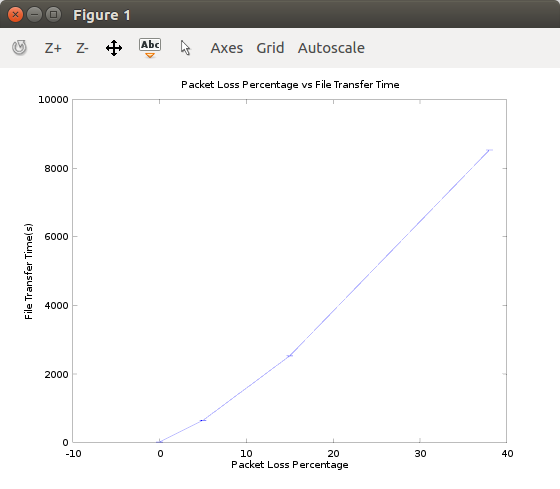
\includegraphics[scale=0.45]{figure.png}
    \caption{Packet Loss Percentage vs File Transfer Time}
\end{figure}

In the graph, you can see the corresponding packet loss values and file transfer time values. We have calculated the standard deviation with the help of standard deviation calculators and in the graph, straight tiny lines represents our error margin.\\

Also, below graph represents the our second experiment findings. It shows the packet loss versus file transfer time relation. Since this experiment was done for only $5\%$ packet loss, only 0 and 5 values are marked here.\\

\begin{figure}[H]
    \centering
    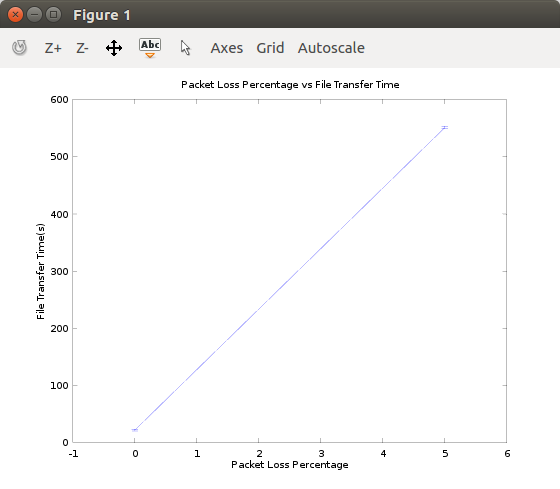
\includegraphics[scale=0.45]{figure2.png}
    \caption{Packet Loss Percentage vs File Transfer Time}
\end{figure}


\end{document}